% !TEX root = Sudoku.tex
% Kapitelvorlage

\section{Einleitung}
\label{sec:Einleitung}
%
\begin{figure}[tb]
    \begin{center}
        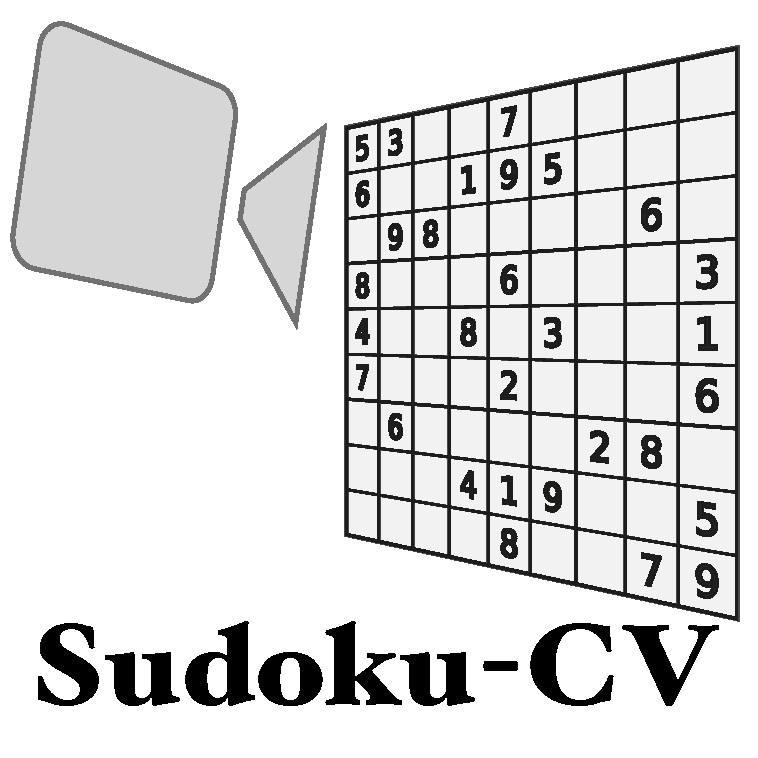
\includegraphics[width=0.4\textwidth]{../Resources/Icon.pdf}
    \end{center}
    \caption{Icon der Anwendung Sudoku-CV}
\end{figure}
%
Als Grundlage dieses Projekts dient das weltweit bekannte Rätsel Sudoku. Dabei handelt es sich um ein 9x9 Gitter, das in neun 3x3 Unterblöcke unterteilt ist.
Ziel ist es das Gitter mit den Ziffern von 1-9 so zu füllen, dass jede Ziffer in jeder neuen Zeile, Spalte und Block nur einmal vorkommt.
Das Ausgangsgitter ist dabei bereits mit einer bestimmten Anzahl an Ziffern ausgefüllt. Je nach Schwierigkeitsgrad kann die Anzahl der ausgefüllten Felder variieren.

Die Software, die in diesem Projekt entwickelt wird, soll das Rätsel mit Hilfe einer Webcam erkennen und simultan lösen.
